% !TEX root = ../main.tex

\section{Firmware Architecture}
\label{sec:firmware-architecture}

\scaffold{
  \textbf{Paragraph 1, language and framework.} The firmware is written in Rust \cite{rust2026} without the standard library and uses the asynchronous Embassy framework \cite{embassy2026} for the RP2350: drivers wait for interrupts as futures, so USB, WiFi, the LEDs and the measurement run as concurrent tasks on one core. The source is in the project repository \cite{benson2026expad}. One sentence on why this matters for the report: a stalled task cannot block the measurement, which became relevant for USB (\cref{sec:output}).
}

\scaffold{
  \textbf{Paragraph 2, two crates and their layers.} Walk through the layers: \code{board} is the only module that knows the PCB (pins, chips, which ADC channel reads which contact); the hardware abstraction layer drives chips (AD7718, shift registers and switches, LEDs, USB, WiFi) without knowing jacks; the scanner runs the measurement on the hardware; the separate library \code{expad-topology} holds the solver arithmetic of \cref{ch:measurement-principle} and the per-jack state machine and knows neither board nor chips. Present \cref{fig:firmware-overview} as the overview of the state machine's four stages and the output.
}

\begin{figure}[htbp]
  \centering
  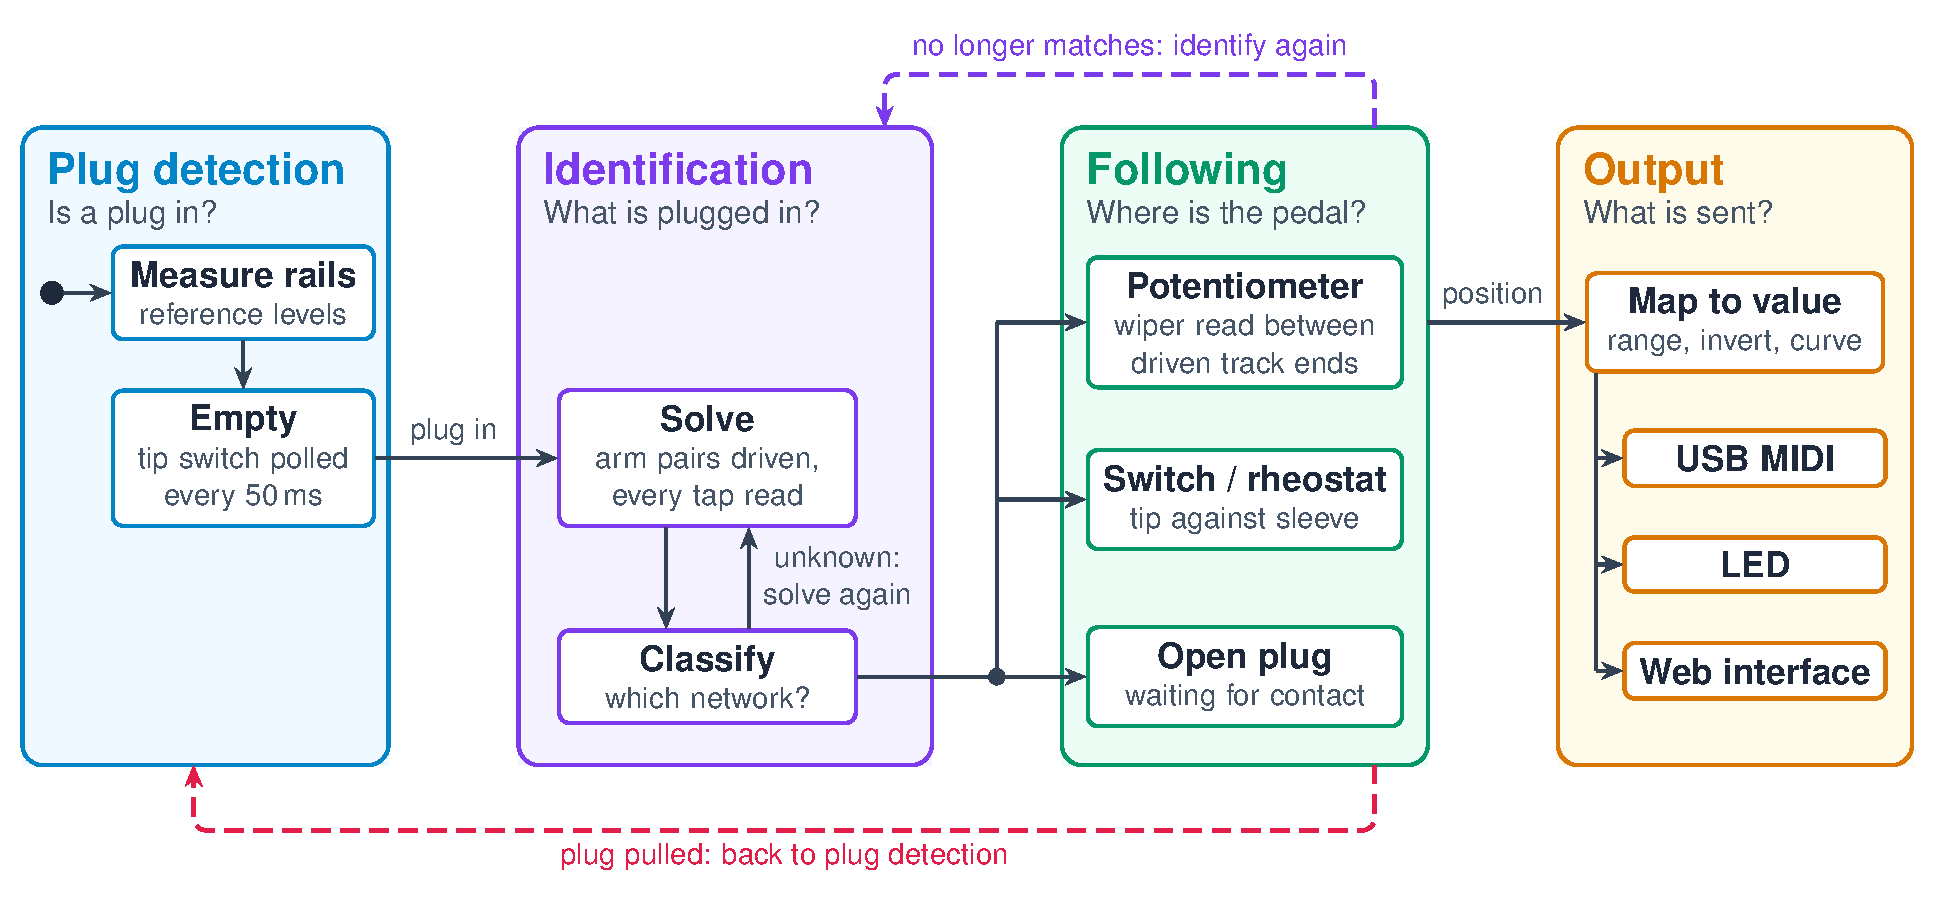
\includegraphics[width=\linewidth]{04-implementation/figures/jack-monitor-overview}
  \titledcaption{Firmware Overview}{\scaffoldinline{Name the four stages per jack (plug detection, identification, following, output) and the two ways back (re-identification when the pedal no longer matches, plug detection when the plug is pulled). Source: \code{docs/diagrams/jack-monitor-overview.tex}.}}
  \label{fig:firmware-overview}
\end{figure}

\scaffold{
  \textbf{Paragraph 3, development on the host.} The solver was first developed in an interactive simulator in TypeScript, shown at milestone~2 \cite{benson2026topologysim}, and then ported to Rust. Because \code{expad-topology} has no hardware dependency, it compiles for the host, where its tests drive the solver against a simulated star network and the state machine against a simulated jack in simulated time (52 tests at the final state, covering plugging, unplugging, end stops, mono and stereo plugs, switches, rheostats, resistive wipers and noise). Give the example that justified this effort: the tests ported from the simulator showed that the first port drove the pairs with high and low swapped, which half of the tests detected before the code ever ran on hardware. Every later solver fix in this report came with a test that fails without it.
}

\scaffold{
  \textbf{Paragraph 4, board-level tools.} Besides the controller firmware, the repository contains small programs that each run on the board alone, the most important being the pin-mapping self-test (\cref{sec:results-self-test}), a capture tool that holds a drive pattern and records every ADC input, and the ADC characterization of \cref{sec:update-rate}. Refer to \cref{tab:binaries} in the appendix for the full list.
}
